\subsection{The Datalogger}
\paragraph{Basic functions \cite{cmp1}}
Simplifying, the CR1000 Datalogger can read data from sensors connected to both its digital and analog pins and store them in tables in its flash (EEPROM) memory.
\begin{figure}
	\centering
	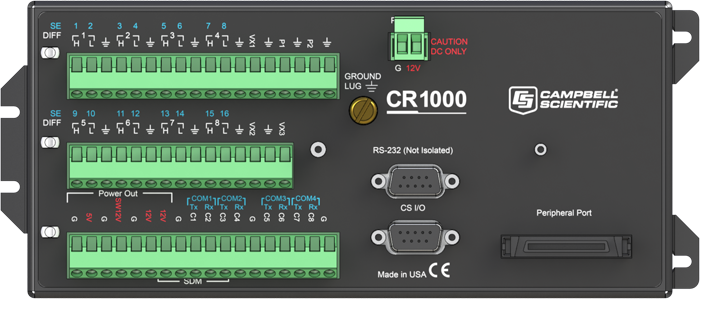
\includegraphics[width=\textwidth]{cr1000_front}
	\caption{CR1000 Datalogger}
	\label{fig:cr1000}
\end{figure}
\paragraph{Sensors on board \cite{avv1}}
The datalogger has the role to enable sensors by giving them power and acquiring measurements form them. The sensors connected to the datalogger at the moment are:
\begin{itemize}
    \item Anemometer: Pulse sensor that measures wind speed and direction
    \item Nivometer: Sonic sensor that measures snow height
    \item Albedometer: Solar radiation
    \item Thermo-Igrometer: Air temperature and humidity
    \item Pirgeometer: IN/OUT long-wavelength radiation
    \item Thermistors: Temperature from Thermo-Igrometer shields
\end{itemize}
\paragraph{Programming}
Actions and table definitions are specified in a source file written in a custom version of BASIC called CRBASIC. Then the program is flashed into the datalogger's memory and it's executed when the device is switched on. The code is shown in appendix \ref{appendix:fcode}
\paragraph{Energy harvesting}
The main concern about the deployment of the datalogger is the energy supply management; in fact the device has a limited power storage provided by a 12V battery but it has to be energy autonomous. However the datalogger has the capability to harvest energy from its solar panel. So it's possible to code programs that run on the device and respect the following energy constraint \cite{avv1}:
\begin{equation}
    E_{harvested}(\Delta t) \geq E_{consumed}(\Delta t)
\end{equation}